\documentclass{beamer}

\usepackage{qtree}
\usepackage{tikz}
\usepackage[UKenglish]{isodate}
\usetikzlibrary{arrows,calc,decorations.pathreplacing,matrix,shapes,mindmap,trees}
\usecolortheme{dove} 
\setbeamertemplate{navigation symbols}{}

\newcommand{\nonterm}[1]{$\left<#1\right>$}
\newcommand{\galt}[0]{$|$}
\newcommand{\kw}[1]{{\bf \texttt{#1}}}
\newcommand{\mkw}[1]{{\bf \mathtt{#1}}}
\newcommand{\sym}[1]{\texttt{#1}}
\newcommand{\msym}[1]{\mathtt{#1}}
\newcommand{\hr}[0]{\rule{10.75cm}{0.4pt}\\}
\newcommand{\centeredtab}[1]{\begin{center}\parbox{0cm}{\begin{tabbing}#1\end{tabbing}}\end{center}}
\def\squareborder#1{\tikz\node[draw]{#1};} 

\pgfarrowsdeclarecombine{twostealth}{twostealth}%
{stealth}{stealth}{stealth}{stealth}

\begin{document}

\title{Introduction to Lambda Calculus}
\author{Maciek Makowski (@mmakowski)}

% -------------------------------------------
\frame{\titlepage}
% -------------------------------------------
\begin{frame}{The Plan}
\begin{center}
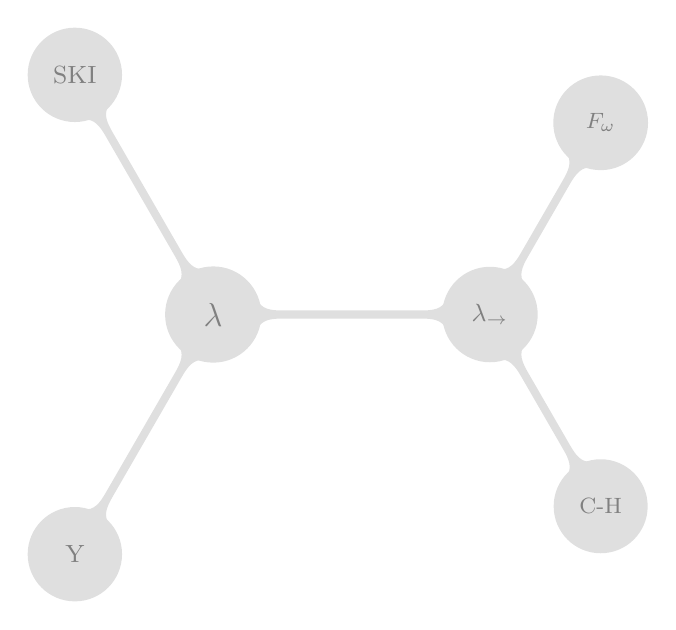
\begin{tikzpicture}
\path[mindmap, 
      concept color=lightgray!50!white,text=gray,
      every node/.style={minimum size=0pt,text width=30pt},
      level 1 concept/.append style={level distance=100,sibling angle=120},
      level 2 concept/.append style={level distance=80,sibling angle=120}
     ]
    node[concept] {$\lambda$}
    [clockwise from=0]
    child[concept] {
      node[concept] {$\lambda_\rightarrow$}
      [clockwise from=60]
      child { node[concept] {$F_\omega$} }
      child { node[concept] {C-H} }
    }  
    child[concept] { node[concept] {Y} }
    child[concept] { node[concept] {SKI} };
\end{tikzpicture}
\end{center}
\end{frame}
% -------------------------------------------
\begin{frame}{Basic Lambda Calculus}
\begin{center}
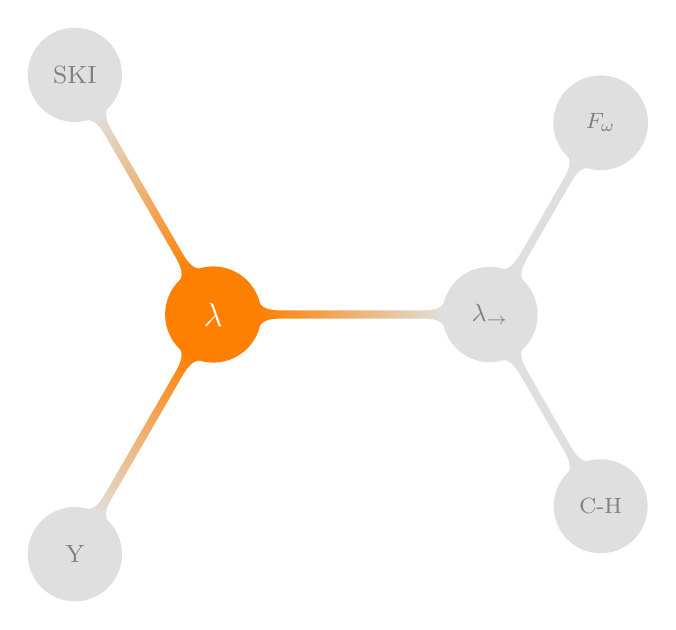
\begin{tikzpicture}
\path[mindmap, 
      concept color=orange,text=white,
      every node/.style={minimum size=0pt,text width=30pt},
      level 1 concept/.append style={level distance=100,sibling angle=120},
      level 2 concept/.append style={level distance=80,sibling angle=120}
     ]
    node[concept] {$\lambda$}
    [clockwise from=0]
    child[concept color=lightgray!50!white,text=gray] {
      node[concept] {$\lambda_\rightarrow$}
      [clockwise from=60]
      child { node[concept] {$F_\omega$} }
      child { node[concept] {C-H} }
    }  
    child[concept color=lightgray!50!white,text=gray] { node[concept] {Y} }
    child[concept color=lightgray!50!white,text=gray] { node[concept] {SKI} };
\end{tikzpicture}
\end{center}
\end{frame}
% -------------------------------------------
\begin{frame}{Syntax}
\begin{tabbing}
\nonterm{term} \= ::=  \= $x$~~~~~~~~~~~~~~~~~~~~~~~~~~~~  \= (variable)    \\
               \> \galt \> ($\lambda x.$\nonterm{term})    \> (abstraction) \\
               \> \galt \> (\nonterm{term} \nonterm{term}) \> (application) 
\end{tabbing}
where $x\in \mathbb{X}$ -- the set of variables

\end{frame}
% -------------------------------------------
\begin{frame}{Syntax}
\begin{tabbing}
~~~~~~~~~~~~~~~~~~~~~~~~~~~~~~~~~~ \= ~~~~~~~~~~~~~~~~~~~~~~~~~~~~~~~~~~~~ \\
$v_1$                              \>                                      \\
\end{tabbing}
\end{frame}
% -------------------------------------------
\begin{frame}{Syntax}
\begin{tabbing}
~~~~~~~~~~~~~~~~~~~~~~~~~~~~~~~~~~ \= ~~~~~~~~~~~~~~~~~~~~~~~~~~~~~~~~~~~~ \\
$v_1$                              \> \Tree [.{var $v_1$} ]                \\
\end{tabbing}
\end{frame}
% -------------------------------------------
\begin{frame}{Syntax}
\begin{tabbing}
~~~~~~~~~~~~~~~~~~~~~~~~~~~~~~~~~~ \= ~~~~~~~~~~~~~~~~~~~~~~~~~~~~~~~~~~~~ \\
$x\ y$                 \>                                      \\
\end{tabbing}
\end{frame}
% -------------------------------------------
\begin{frame}{Syntax}
\begin{tabbing}
~~~~~~~~~~~~~~~~~~~~~~~~~~~~~~~~~~ \= ~~~~~~~~~~~~~~~~~~~~~~~~~~~~~~~~~~~~ \\
$x\ y$                             \> \Tree [.app {var $x$} {var $y$} ]    \\
\end{tabbing}
\end{frame}
% -------------------------------------------
\begin{frame}{Syntax}
\begin{tabbing}
~~~~~~~~~~~~~~~~~~~~~~~~~~~~~~~~~~ \= ~~~~~~~~~~~~~~~~~~~~~~~~~~~~~~~~~~~~ \\
$\lambda a.b$                      \>                                      \\
\end{tabbing}
\end{frame}
% -------------------------------------------
\begin{frame}{Syntax}
\begin{tabbing}
~~~~~~~~~~~~~~~~~~~~~~~~~~~~~~~~~~ \= ~~~~~~~~~~~~~~~~~~~~~~~~~~~~~~~~~~~~ \\
$\lambda a.b$                      \> \Tree [.{abs $a$} {var $b$} ]        \\
\end{tabbing}
\end{frame}
% -------------------------------------------
\begin{frame}{Syntax}
\begin{tabbing}
~~~~~~~~~~~~~~~~~~~~~~~~~~~~~~~~~~ \= ~~~~~~~~~~~~~~~~~~~~~~~~~~~~~~~~~~~~ \\
$(\lambda a.\lambda b.a)\ c\ (\lambda b.b)$ \>                             \\
\end{tabbing}
\end{frame}
% -------------------------------------------
\begin{frame}{Syntax}
\begin{tabbing}
\nonterm{term} \= ::=  \= $x$~~~~~~~~~~~~~~~~~~~~~~~~~~~~  \= (variable)    \\
               \> \galt \> ($\lambda x.$\nonterm{term})    \> (abstraction) \\
               \> \galt \> (\nonterm{term} \nonterm{term}) \> (application) 
\end{tabbing}
\end{frame}
% -------------------------------------------
\begin{frame}{Syntax}
\begin{tabbing}
~~~~~~~~~~~~~~~~~~~~~~~~~~~~~~~~~~ \= ~~~~~~~~~~~~~~~~~~~~~~~~~~~~~~~~~~~~ \\
$(\lambda a.\lambda b.a)\ c\ (\lambda b.b)$ \> \Tree [.app [.app [.{abs $a$} 
[.{abs $b$} {var $a$} ] ] {var $c$} ] [.{abs $b$} {var $b$} ] ]             \\
\end{tabbing}
\end{frame}
% -------------------------------------------
\begin{frame}{Syntax}
\begin{tabbing}
~~~~~~~~~~~~~~~~~~~~~~~~~~~~~~~~~~ \= ~~~~~~~~~~~~~~~~~~~~~~~~~~~~~~~~~~~~ \\
$(\lambda a.b\ a)\ c\ (\lambda b.b)$  \> 
\Tree [.app [.app [.{abs $a$} 
[.app {var $b$} {var $a$} ] ] {var $c$} ] [.{abs $b$} {var $b$} ] ]            \\
\end{tabbing}
\end{frame}
% -------------------------------------------
\begin{frame}{Syntax}
\begin{tabbing}
~~~~~~~~~~~~~~~~~~~~~~~~~~~~~~~~~~ \= ~~~~~~~~~~~~~~~~~~~~~~~~~~~~~~~~~~~~ \\
$(\lambda a.\underline{b}\ a)\ \underline{c}\ (\lambda b.b)$ \> 
\Tree [.app [.app [.{abs $a$} [.app \squareborder{var $b$} {var $a$} ] ] 
\squareborder{var $c$} ] [.{abs $b$} {var $b$} ] ]            \\
\end{tabbing}
\end{frame}
% -------------------------------------------
\begin{frame}{Syntax}
\begin{itemize}
\item terms: trees consisting of 
\begin{itemize}
\item variables
\item abstractions
\item applications
\end{itemize}
\item variables are \textit{bound} by abstraction; otherwise \textit{free}
\end{itemize}
\end{frame}
% -------------------------------------------
\begin{frame}{Rewriting}{$\alpha$-conversion}
\begin{align*}
(\lambda x.x\,y)\ (\lambda x.x)\longleftrightarrow_\alpha(\lambda a.a\,y)\ (\lambda b.b)
\end{align*}
\end{frame}
% -------------------------------------------
\begin{frame}{Rewriting}{$\beta$-reduction}
\begin{align*}
(\lambda x.M)\ N\longrightarrow_\beta M[x/N]
\end{align*}
\end{frame}
% -------------------------------------------
\begin{frame}{Rewriting}{$\beta$-reduction}
\begin{align*}
(\lambda x.M)\ N\longrightarrow_\beta M[x/N] \\
\end{align*}
\hr
\begin{align*}
(\lambda x.x\,y)\ (\lambda z.z)\longrightarrow_\beta(\lambda z.z)\ y\longrightarrow_\beta y
\end{align*}
\end{frame}
% -------------------------------------------
\begin{frame}{Rewriting}{$\beta$-reduction}
\begin{itemize}
\item \textit{call-by-value}: start with innermost redex, do not reduce under abstraction
\item \textit{call-by-name}: start with outermost redex, do not reduce under abstraction
\end{itemize}
\end{frame}
% -------------------------------------------
\begin{frame}{Rewriting}{Church-Rosser}
\begin{center}
\begin{tikzpicture}[->,>=twostealth,node distance=2cm]
    \node(S) {$S$};
    \node(T) [below left of=S] {$T$};
    \node(U) [below right of=S] {$U$};
    \node(V) [below left of=U] {$V$};
    \draw (S) -- (T);
    \draw (S) -- (U);
    \draw[densely dotted] (T) -- (V);
    \draw[densely dotted] (U) -- (V);
\end{tikzpicture}
\end{center}
\end{frame}
% -------------------------------------------
\begin{frame}{Semantics}
\begin{align*}
f(x)=3*x+2 \\
\phantom{\lambda x.+\,(*\,3\,x)\,2}
\end{align*}
\end{frame}
% -------------------------------------------
\begin{frame}{Semantics}
\begin{align*}
f(x)=3*x+2 \\
\lambda x.+\,(*\,3\,x)\,2
\end{align*}
\end{frame}
% -------------------------------------------
\begin{frame}{Programming in Lambda Calculus}
\begin{center}
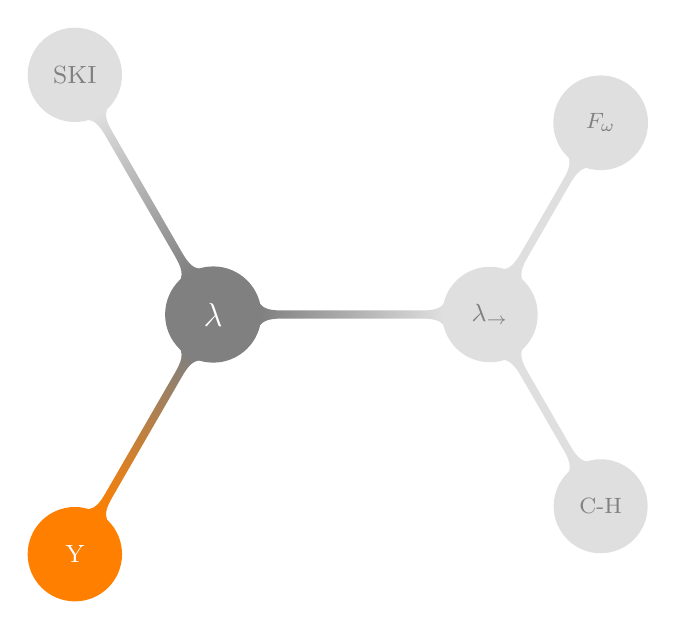
\begin{tikzpicture}
\path[mindmap, 
      concept color=gray,text=white,
      every node/.style={minimum size=0pt,text width=30pt},
      level 1 concept/.append style={level distance=100,sibling angle=120},
      level 2 concept/.append style={level distance=80,sibling angle=120}
     ]
    node[concept] {$\lambda$}
    [clockwise from=0]
    child[concept color=lightgray!50!white,text=gray] {
      node[concept] {$\lambda_\rightarrow$}
      [clockwise from=60]
      child { node[concept] {$F_\omega$} }
      child { node[concept] {C-H} }
    }  
    child[concept color=orange] { node[concept] {Y} }
    child[concept color=lightgray!50!white,text=gray] { node[concept] {SKI} };
\end{tikzpicture}
\end{center}
\end{frame}
% -------------------------------------------
\begin{frame}{Conditionals}
\begin{center}
\kw{if} $C$ \kw{then} $T$ \kw{else} $F$
\end{center}
\hr
\begin{align*}
\phantom{\msym{true}  &= \lambda t.\lambda f.t} \\
\phantom{\msym{false} &= \lambda t.\lambda f.f} \\
\phantom{\msym{test} &= \lambda c.\lambda t.\lambda f.c\,t\,f} \\
\phantom{\mkw{if}\,C\,\mkw{then}\,T\,\mkw{else}\,F &= \msym{test}\,C\,T\,F}
\end{align*}
\end{frame}
% -------------------------------------------
\begin{frame}{Conditionals}
\begin{center}
\kw{if} $C$ \kw{then} $T$ \kw{else} $F$
\end{center}
\hr
\begin{align*}
\msym{true}  &= \lambda t.\lambda f.t \\
\msym{false} &= \lambda t.\lambda f.f
\phantom{\msym{test} &= \lambda c.\lambda t.\lambda f.c\,t\,f} \\
\phantom{\mkw{if}\,C\,\mkw{then}\,T\,\mkw{else}\,F &= \msym{test}\,C\,T\,F}
\end{align*}
\end{frame}
% -------------------------------------------
\begin{frame}{Conditionals}
\begin{center}
\kw{if} $C$ \kw{then} $T$ \kw{else} $F$
\end{center}
\hr
\begin{align*}
\msym{true}  &= \lambda t.\lambda f.t \\
\msym{false} &= \lambda t.\lambda f.f \\
\msym{test} &= \lambda c.\lambda t.\lambda f.c\,t\,f \\
\mkw{if}\,C\,\mkw{then}\,T\,\mkw{else}\,F &= \msym{test}\,C\,T\,F
\end{align*}
\end{frame}
% -------------------------------------------
\begin{frame}{Conditionals}
\begin{center}
\kw{if} $C$ \kw{then} $T$ \kw{else} $F$
\end{center}
\hr
\begin{align*}
\msym{true}  &= \lambda t.\lambda f.t \\
\msym{false} &= \lambda t.\lambda f.f \\
\msym{test} &= \lambda c.\lambda t.\lambda f.c\,t\,f \\
\mkw{if}\,C\,\mkw{then}\,T\,\mkw{else}\,F &= \msym{test}\,C\,T\,F
\end{align*}
\end{frame}
% -------------------------------------------
\begin{frame}{Numbers}
\begin{align*}
\msym{0}    &= \lambda s.\lambda z.z \\
\msym{succ} &= \lambda n.\lambda s.\lambda z.s\,(n\,s\,z)
\end{align*}
\end{frame}
% -------------------------------------------
\begin{frame}{Numbers}
\begin{align*}
\msym{0}    &= \lambda s.\lambda z.z \\
\msym{succ} &= \lambda n.\lambda s.\lambda z.s\,(n\,s\,z)
\end{align*}
\centeredtab{
\sym{0} \= $=$ \= ~~~~~~~~~    \= ~~~ \= $\lambda s.\lambda z.z$    \\
\sym{1} \> $=$ \> \sym{succ 0} \> $=$ \> $\lambda s.\lambda z.s\,z$ \\
\sym{2} \> $=$ \> \sym{succ 1} \> $=$ \> $\lambda s.\lambda z.s\,(s\,z)$ \\
\sym{3} \> $=$ \> \sym{succ 2} \> $=$ \> $\lambda s.\lambda z.s\,(s\,(s\,z))$ \\
$\vdots$ \\
\sym{n} \> $=$ \> \> \> $\lambda s.\lambda z\underbrace{s\,(\dots s\,(s}_n\,z)\dots)$
}
\end{frame}
% -------------------------------------------
\begin{frame}{Numbers}
\begin{align*}
\msym{0}    &= \lambda s.\lambda z.z \\
\msym{succ} &= \lambda n.\lambda s.\lambda z.s\,(n\,s\,z)
\end{align*}
\begin{align*}
\msym{plus}  &= \lambda m.\lambda n.\lambda s. \lambda z.m\ s\ (n\ s\ z) \\
\msym{times} &= \lambda m.\lambda n.m\ (\msym{plus}\ n)\ \msym{0}
\end{align*}
\end{frame}
% -------------------------------------------
\begin{frame}{Recursion}
\begin{align*}
n!=\begin{cases}
    1 & \text{if $n=0$},\\
    n*(n-1)! & \text{otherwise}.
  \end{cases}
\end{align*}
\end{frame}
% -------------------------------------------
\begin{frame}{Recursion}
\begin{align*}
\msym{Y} &= \lambda f.(\lambda x.f\,(x\,x))\,(\lambda x.f\,(x\,x)) \\\\
\msym{g} &= \lambda f.\lambda
n.\mkw{if}\ \msym{eq}\ n\ \msym{0}\ \mkw{then}\ \msym{1}\ \mkw{else}\ (\msym{times}\ \msym{n}\,(f\,(\msym{pred}\ \msym{n}))) \\
\msym{factorial} &= \msym{Y}\ \msym{g}
\end{align*}
\end{frame}


% -------------------------------------------
\begin{frame}{Simple Types}
\begin{center}
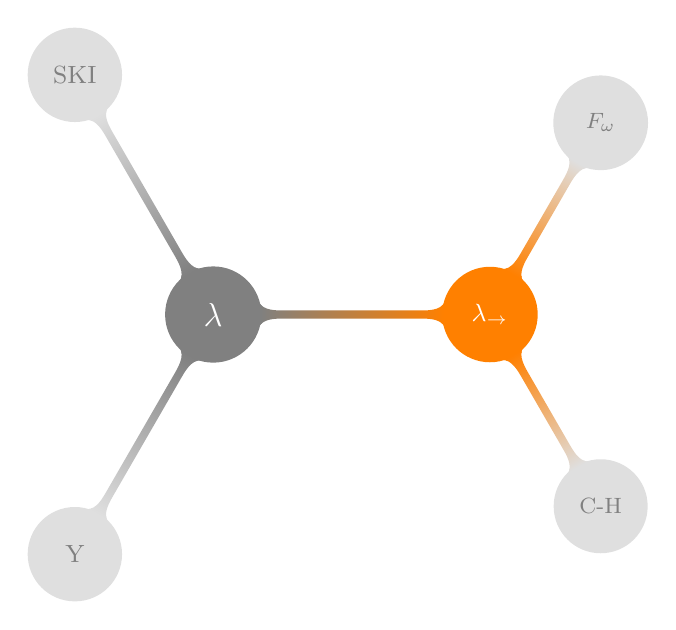
\begin{tikzpicture}
\path[mindmap, 
      concept color=gray,text=white,
      every node/.style={minimum size=0pt,text width=30pt},
      level 1 concept/.append style={level distance=100,sibling angle=120},
      level 2 concept/.append style={level distance=80,sibling angle=120}
     ]
    node[concept] {$\lambda$}
    [clockwise from=0]
    child[concept color=orange] {
      node[concept] {$\lambda_\rightarrow$}
      [clockwise from=60]
      child[concept color=lightgray!50!white,text=gray] { node[concept] {$F_\omega$} }
      child[concept color=lightgray!50!white,text=gray] { node[concept] {C-H} }
    }  
    child[concept color=lightgray!50!white,text=gray] { node[concept] {Y} }
    child[concept color=lightgray!50!white,text=gray] { node[concept] {SKI} };
\end{tikzpicture}
\end{center}
\end{frame}
% -------------------------------------------
\begin{frame}{Curry-Howard Correspondence}
\begin{center}
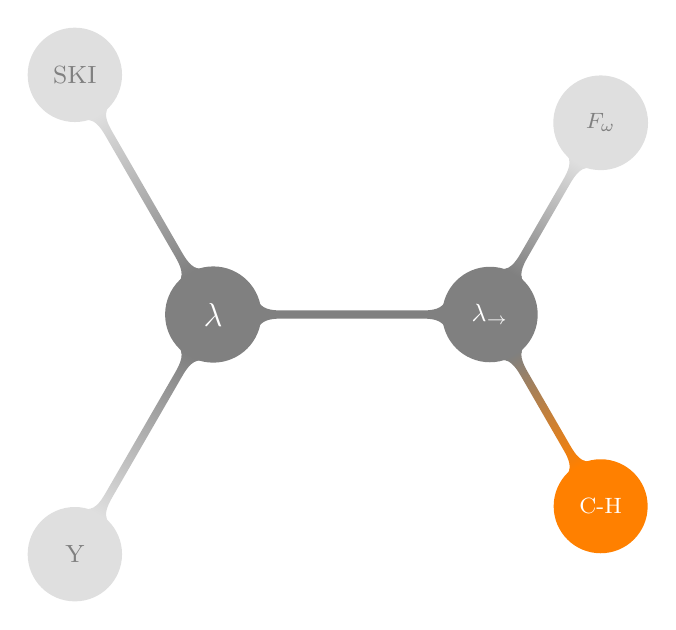
\begin{tikzpicture}
\path[mindmap, 
      concept color=gray,text=white,
      every node/.style={minimum size=0pt,text width=30pt},
      level 1 concept/.append style={level distance=100,sibling angle=120},
      level 2 concept/.append style={level distance=80,sibling angle=120}
     ]
    node[concept] {$\lambda$}
    [clockwise from=0]
    child[concept] {
      node[concept] {$\lambda_\rightarrow$}
      [clockwise from=60]
      child[concept color=lightgray!50!white,text=gray] { node[concept] {$F_\omega$} }
      child[concept color=orange] { node[concept] {C-H} }
    }  
    child[concept color=lightgray!50!white,text=gray] { node[concept] {Y} }
    child[concept color=lightgray!50!white,text=gray] { node[concept] {SKI} };
\end{tikzpicture}
\end{center}
\end{frame}
% -------------------------------------------
\begin{frame}{More Types}
\begin{center}
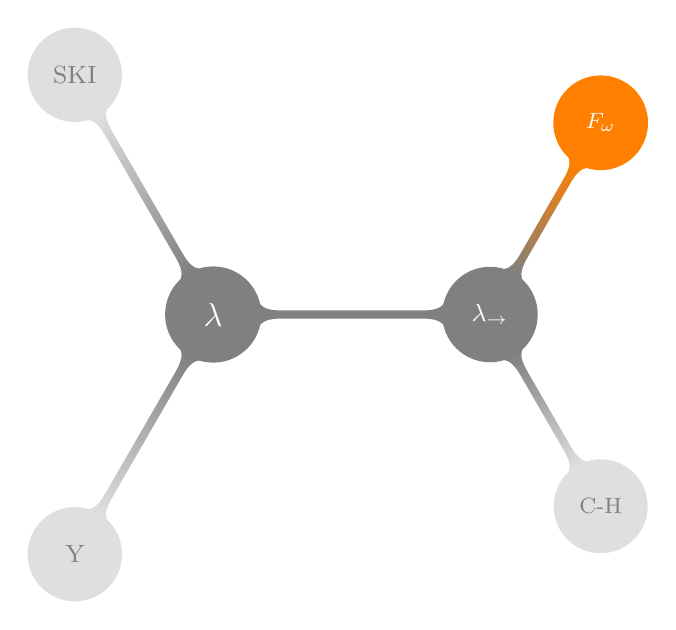
\begin{tikzpicture}
\path[mindmap, 
      concept color=gray,text=white,
      every node/.style={minimum size=0pt,text width=30pt},
      level 1 concept/.append style={level distance=100,sibling angle=120},
      level 2 concept/.append style={level distance=80,sibling angle=120}
     ]
    node[concept] {$\lambda$}
    [clockwise from=0]
    child[concept] {
      node[concept] {$\lambda_\rightarrow$}
      [clockwise from=60]
      child[concept color=orange] { node[concept] {$F_\omega$} }
      child[concept color=lightgray!50!white,text=gray] { node[concept] {C-H} }
    }  
    child[concept color=lightgray!50!white,text=gray] { node[concept] {Y} }
    child[concept color=lightgray!50!white,text=gray] { node[concept] {SKI} };
\end{tikzpicture}
\end{center}
\end{frame}
% -------------------------------------------
\begin{frame}{The Lambda Cube}
\begin{center}
\begin{tikzpicture}
  \matrix(m)[matrix of math nodes, row sep=3em, column sep=3em, ampersand replacement=\&]{
                 \& \vphantom{F^\omega_{<:}}       \&                     \& \vphantom{\lambda\omega}             \&            \& \vphantom{\lambda P\omega}      \\
    \vphantom{F_{<:}}       \&                     \& \lambda 2           \&                           \& \vphantom{\lambda P2} \&                      \\
                 \&                     \&                     \& \lambda\underline{\omega} \&            \& \vphantom{\lambda P\underline{\omega}} \\
    \vphantom{\lambda_{<:}} \&                     \& \lambda_\rightarrow \&                           \& \lambda P  \&                      \\
  };
  \path[-stealth]
    (m-4-3) edge (m-2-3) edge (m-4-5) edge (m-3-4);
\end{tikzpicture}
\end{center}
\end{frame}
% -------------------------------------------
\begin{frame}{The Lambda Cube}
\begin{center}
\begin{tikzpicture}
  \matrix(m)[matrix of math nodes, row sep=3em, column sep=3em, ampersand replacement=\&]{
                 \& \vphantom{F^\omega_{<:}}       \&                     \& \lambda\omega             \&            \& \lambda P\omega      \\
    \vphantom{F_{<:}}       \&                     \& \lambda 2           \&                           \& \lambda P2 \&                      \\
                 \&                     \&                     \& \lambda\underline{\omega} \&            \& \lambda P\underline{\omega} \\
    \vphantom{\lambda_{<:}} \&                     \& \lambda_\rightarrow \&                           \& \lambda P  \&                      \\
  };
  \path[-stealth]
    (m-4-3) edge (m-2-3) edge (m-4-5) edge [densely dotted] (m-3-4)
    (m-3-4) edge [densely dotted] (m-1-4) edge [densely dotted] (m-3-6)
    (m-2-3) edge (m-1-4) edge [-,line width=6pt,draw=white] (m-2-5) edge (m-2-5)
    (m-4-5) edge (m-3-6) edge [-,line width=6pt,draw=white] (m-2-5) edge (m-2-5)
    (m-1-4) edge (m-1-6)
    (m-2-5) edge (m-1-6)
    (m-3-6) edge (m-1-6);
\end{tikzpicture}
\end{center}
\end{frame}
% -------------------------------------------
\begin{frame}{Subtyping}
\begin{center}
\begin{tikzpicture}
  \matrix(m)[matrix of math nodes, row sep=3em, column sep=3em, ampersand replacement=\&]{
                 \& \vphantom{F^\omega_{<:}}       \&                     \& \lambda\omega             \&            \& \lambda P\omega      \\
    \vphantom{F_{<:}}       \&                     \& \lambda 2           \&                           \& \lambda P2 \&                      \\
                 \&                     \&                     \& \lambda\underline{\omega} \&            \& \lambda P\underline{\omega} \\
    \lambda_{<:} \&                     \& \lambda_\rightarrow \&                           \& \lambda P  \&                      \\
  };
  \path[-stealth]
    (m-4-3) edge (m-2-3) edge (m-4-5) edge [densely dotted] (m-3-4)
    (m-3-4) edge [densely dotted] (m-1-4) edge [densely dotted] (m-3-6)
    (m-2-3) edge (m-1-4) edge [-,line width=6pt,draw=white] (m-2-5) edge (m-2-5)
    (m-4-5) edge (m-3-6) edge [-,line width=6pt,draw=white] (m-2-5) edge (m-2-5)
    (m-1-4) edge (m-1-6)
    (m-2-5) edge (m-1-6)
    (m-3-6) edge (m-1-6)
    % end of cube edges
    (m-4-3) edge (m-4-1);
\end{tikzpicture}
\end{center}
\end{frame}
% -------------------------------------------
\begin{frame}{Subtyping}
\begin{center}
\begin{tikzpicture}
  \matrix(m)[matrix of math nodes, row sep=3em, column sep=3em, ampersand replacement=\&]{
                 \& F^\omega_{<:}       \&                     \& \lambda\omega             \&            \& \lambda P\omega      \\
    F_{<:}       \&                     \& \lambda 2           \&                           \& \lambda P2 \&                      \\
                 \&                     \&                     \& \lambda\underline{\omega} \&            \& \lambda P\underline{\omega} \\
    \lambda_{<:} \&                     \& \lambda_\rightarrow \&                           \& \lambda P  \&                      \\
  };
  \path[-stealth]
    (m-4-3) edge (m-2-3) edge (m-4-5) edge [densely dotted] (m-3-4)
    (m-3-4) edge [densely dotted] (m-1-4) edge [densely dotted] (m-3-6)
    (m-2-3) edge (m-1-4) edge [-,line width=6pt,draw=white] (m-2-5) edge (m-2-5)
    (m-4-5) edge (m-3-6) edge [-,line width=6pt,draw=white] (m-2-5) edge (m-2-5)
    (m-1-4) edge (m-1-6)
    (m-2-5) edge (m-1-6)
    (m-3-6) edge (m-1-6)
    % end of cube edges
    (m-4-3) edge (m-4-1)
    (m-4-1) edge (m-2-1)
    (m-2-3) edge (m-2-1)
    (m-2-1) edge (m-1-2)
    (m-1-4) edge (m-1-2);
\end{tikzpicture}
\end{center}
\end{frame}
% -------------------------------------------

\end{document}
